\documentclass[8pt,a4paper,compress]{beamer}

\usepackage{/home/siyer/lib/slides}

\title{Directed Graphs}
\date{}
\begin{document}
\begin{frame}
\vfill
\titlepage
\end{frame}

\section{Directed Graphs}
\begin{frame}[fragile]
\pause

\begin{minipage}{170pt}
A directed graph (digraph) is a set of vertices and a collection of directed edges, each connecting an ordered pair of vertices

\pause
\bigskip

The outdegree of a vertex in a digraph is the number of edges
going from it; the indegree of a vertex is the number of edges going to it

\pause
\bigskip

A directed path in a digraph is a sequence of vertices in which there is a (directed) edge pointing from each vertex in the sequence to its successor in the sequence

\pause
\bigskip

A directed cycle is a directed path with at least one edge whose first and last vertices are the same

\pause
\bigskip

The length of a path or a cycle is its number of edges
\end{minipage}%
\begin{minipage}{130pt}
\begin{center}
\hfill \visible<2->{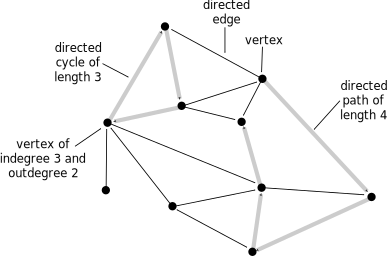
\includegraphics[scale=0.39]{{./figures/digraph1}.pdf}}
\end{center}
\end{minipage}
\end{frame}

\begin{frame}[fragile]
\pause

Digraph applications
\begin{center}
\begin{tabular}{ccc}
digraph & vertex & edge \\ \hline
transportation & street intersection & one-way street \\
web & web page & hyperlink \\
food web & species & predator-prey relationship \\
WordNet & synset & hypernym \\
scheduling & task & precedence constraint \\
financial & bank & transaction \\
cell phone & person & placed call \\
infectious disease & person & infection \\
game & board position & legal move \\
citation & journal article & citation \\
object graph & object & pointer \\
inheritance hierarchy & class & inherits from \\ 
control flow & code block & jump
\end{tabular}  
\end{center}
\end{frame}

\begin{frame}[fragile]
\pause

Some digraph problems
\begin{center}
\begin{tabular}{cc}
problem & description \\ \hline
$s\to t$ path & is there a path from $s$ to $t$? \\ 
shortest $s\to t$ path & what is the shortest path from $s$ to $t$? \\
directed cycle & is there a directed cycle in the graph? \\
topological sort & \makecell{can the digraph be drawn so that all \\ edges point in a single direction?} \\
strong connectivity & is there a directed path between all pairs of vertices? \\
transitive closure & \makecell{for which vertices $v$ and $w$ is there a \\ directed path from $v$ to $w$?} \\
page rank & what is the importance of a web page?
\end{tabular}  
\end{center}
\end{frame}

\begin{frame}[fragile]
\pause

Digraph API

\begin{center}
\begin{tabular}{cc}
method & description \\ \hline
\lstinline$Digraph(int V)$ & create an empty digraph with $V$ vertices \\
\lstinline$Digraph(In in)$ & create a digraph from input stream \\
\lstinline$void addEdge(int v, int w)$ & add a directed edge $v \to w$ \\
\lstinline$Iterable<Integer> adj(int v)$ & vertices pointing from $v$ \\
\lstinline$int V()$ & number of vertices \\
\lstinline$int E()$ & number of edges \\
\lstinline$Digraph reverse()$ & reverse of this digraph
\end{tabular} 
\end{center}

\pause
\bigskip

Graph input format
\begin{minipage}{150pt}
\begin{lstlisting}[language={},style=focusin]
$ more tinyDG.txt
13 22 
4 2 2 3 3 2 6 0 0 1 2 0 11 12 12 9
9 10 9 11 8 9 10 12 11 4 4 3 3 5
7 8 8 7 5 4 0 5 6 4 6 9 7 6
\end{lstlisting}
\end{minipage}%
\begin{minipage}{150pt}
\begin{center}
\visible<3->{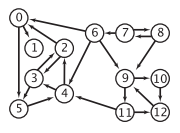
\includegraphics[scale=0.4]{{./figures/digraph2}.pdf}}
\end{center}
\end{minipage}

\pause
\bigskip

Typical graph-processing code
\begin{lstlisting}[language=java,style=focusin]
In in = new In(args[0]);
Digraph G = new Digraph(in);
for (int v = 0; v < G.V(); v++) {
    for (int w : G.adj(v)) {
        StdOut.println(v + "->" + w);
    }
}
\end{lstlisting}
\end{frame}

\begin{frame}[fragile]
\pause

Implementation of \lstinline{Digraph} data type using an adjacency list
\begin{lstlisting}[language=java,style=focusin]
package edu.princeton.cs.algs4;

import java.util.InputMismatchException;
import java.util.NoSuchElementException;

public class Digraph {
    private final int V;
    private int E;
    private LinkedBag<Integer>[] adj;

    public Digraph(int V) {
        if (V < 0) { throw new IllegalArgumentException(); }
        this.V = V;
        this.E = 0;
        adj = (LinkedBag<Integer>[]) new LinkedBag[V];
        for (int v = 0; v < V; v++) { 
            adj[v] = new LinkedBag<Integer>(); 
        }
    }

    public Digraph(In in) {
        this(in.readInt());
        int E = in.readInt();
        if (E < 0) { throw new IllegalArgumentException(); }
        for (int i = 0; i < E; i++) {
            int v = in.readInt();
            int w = in.readInt();
            addEdge(v, w); 
        }
    }
\end{lstlisting}
\end{frame}

\begin{frame}[fragile]
\pause

\begin{lstlisting}[language=java,style=focusin]
    public int V() { return V; }

    public int E() { return E; }

    private void validateVertex(int v) {
        if (v < 0 || v >= V) { throw new IndexOutOfBoundsException(); }
    }

    public void addEdge(int v, int w) {
        validateVertex(v);
        validateVertex(w);
        adj[v].add(w);
        E++;
    }

    public Iterable<Integer> adj(int v) {
        validateVertex(v);
        return adj[v];
    }

    public Digraph reverse() {
        Digraph R = new Digraph(V);
        for (int v = 0; v < V; v++) {
            for (int w : adj(v)) {
                R.addEdge(w, v);
            }
        }
        return R;
    }
}
\end{lstlisting}
\end{frame}

\section{Depth-First Search (DFS)}
\begin{frame}[fragile]
\pause

Same method as for undirected graphs, ie, to visit a vertex $v$
\begin{itemize}
\item Mark a vertex $v$ as visited

\item Recursively visit all unmarked vertices pointing from $v$
\end{itemize}

\pause
\bigskip

Reachability problem
\begin{itemize}
\item Single-source reachability: given a digraph and a source vertex $s$, support queries of the form \emph{is there a directed path from $s$ to a given target vertex $v$?}

\item Multi-source reachability: given a digraph and a set of source vertices, support queries of the form \emph{is there a directed path from any vertex in the set to a given target vertex $v$?}
\end{itemize}

\pause
\bigskip

Applications
\begin{itemize}
\item Program control-flow analysis such as dead-code elimination and  infinite-loop detection

\item Mark and sweep garbage collector
\end{itemize}
\end{frame}

\section{Breadth-First Search (BFS)}
\begin{frame}[fragile]
\pause

Same method as for undirected graphs, ie, repeat until queue is empty
\begin{itemize}
\item Remove vertex $v$ from queue

\item Add to queue all unmarked vertices pointing from $v$ and mark them
\end{itemize}

\pause
\bigskip

BFS computes shortest paths (fewest number of edges)
from source vertex $s$ to all other vertices in a digraph in time proportional to $E + V$

\pause
\bigskip

Multiple-source shortest paths: given a digraph and a set of source vertices, find shortest path from any vertex in the set to each other vertex; solution: use BFS, but initialize by enqueuing all source vertices
\end{frame}

\begin{frame}[fragile]
\pause

Application (web crawler)
\begin{lstlisting}[language=java,style=focusin]
import edu.princeton.cs.algs4.*;
import java.util.regex.*;

public class WebCrawler { 
    public static void main(String[] args) { 
        String s = args[0];
        LinkedQueue<String> queue = new LinkedQueue<String>();
        queue.enqueue(s);
        SET<String> marked = new SET<String>();
        marked.add(s);
        while (!queue.isEmpty()) {
            String v = queue.dequeue();
            System.out.println(v);
            In in = new In(v);
            if (!in.exists()) { continue; }
            String input = in.readAll();
            if (input == null) { continue; }
            String regexp = "http://(\\w+\\.)+(\\w+)";
            Pattern pattern = Pattern.compile(regexp);
            Matcher matcher = pattern.matcher(input);
            while (matcher.find()) {
                String w = matcher.group();
                if (!marked.contains(w)) { queue.enqueue(w); marked.add(w); }
            }
        }
    }
}
\end{lstlisting}

\pause

\begin{lstlisting}[language={},style=focusin]
$ java WebCrawler http://www.swamiiyer.net/
http://www.swamiiyer.net/
http://www.w3.org
http://jemdoc.jaboc.net
...
\end{lstlisting}
\end{frame}

\section{Topological Sort}
\begin{frame}[fragile]
\pause

Precedence-constrained scheduling: given a set of jobs to be completed, with precedence constraints that specify that certain jobs have to be completed before certain other jobs are begun, how can we schedule the jobs such that they are all completed while still respecting the constraints?

\pause
\bigskip

Example (precedence-constrained course scheduling problem)
\begin{center}
\visible<3->{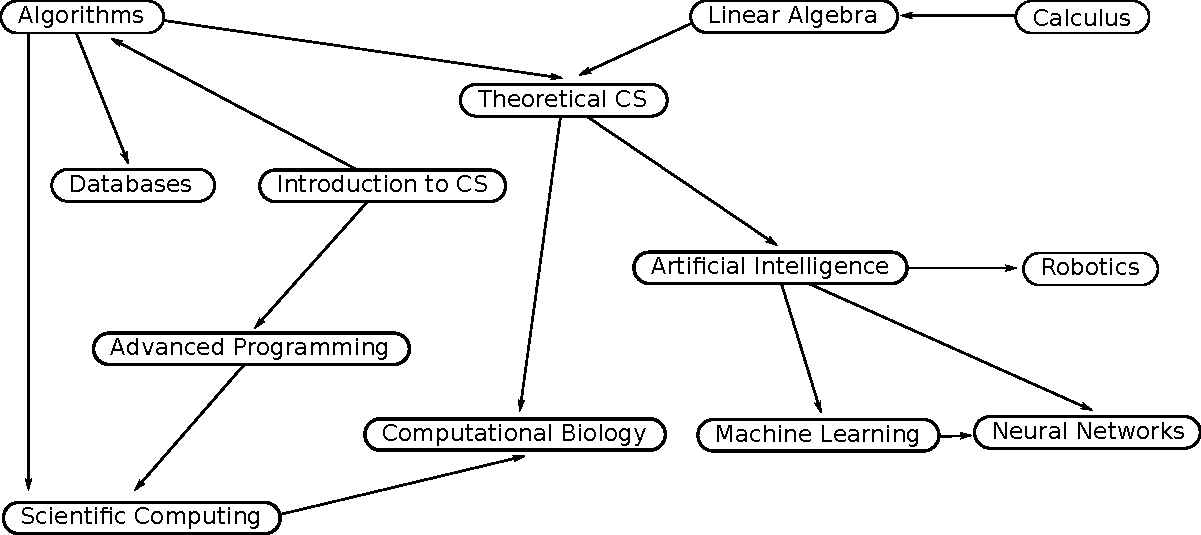
\includegraphics[scale=0.35]{{./figures/digraph3}.pdf}}
\end{center}

\pause
\bigskip

A digraph model for the problem
\begin{center}
\visible<4->{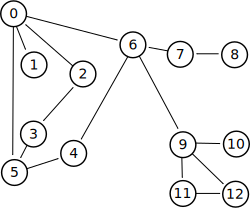
\includegraphics[scale=0.35]{{./figures/digraph4}.pdf}}
\end{center}
\end{frame}

\begin{frame}[fragile]
\pause

Topological sort: given a directed acyclic graph (DAG), put the vertices in order such that all its edges point from a vertex earlier in the order to a vertex later in the order

\pause
\bigskip

A digraph has a topological order if and only if it is a DAG

\pause
\bigskip

Topological order for the precedence-constrained course scheduling problem
\begin{center}
\visible<4->{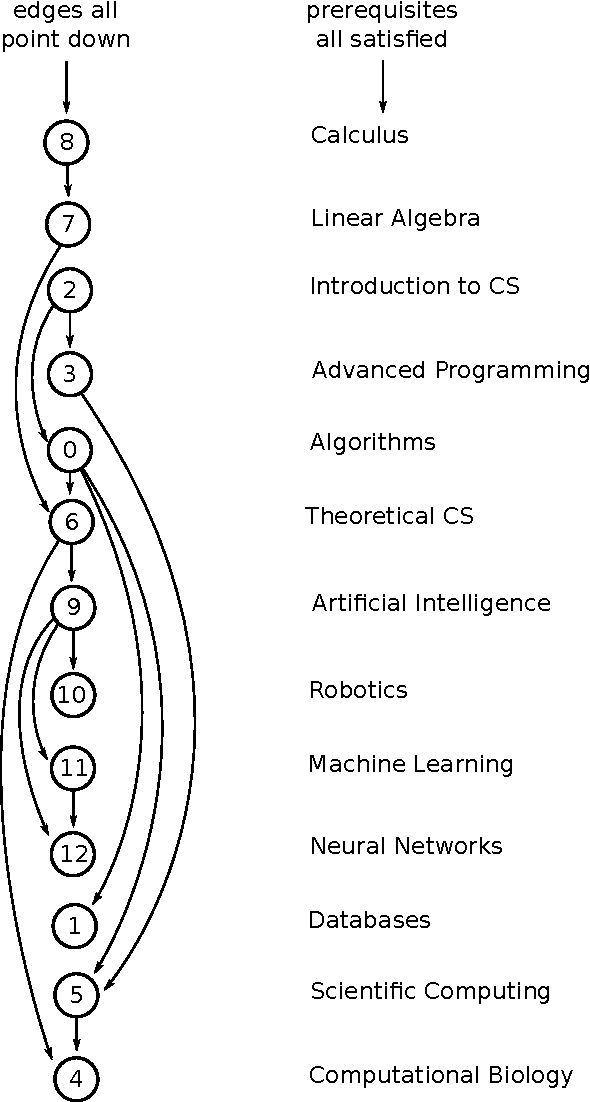
\includegraphics[scale=0.35]{{./figures/digraph5}.pdf}}
\end{center}
\end{frame}

\begin{frame}[fragile]
\pause

Directed cycle detection
\begin{lstlisting}[language=java,style=focusin]
package edu.princeton.cs.algs4;

public class DirectedCycle {
    private boolean[] marked; 
    private int[] edgeTo; 
    private boolean[] onStack; 
    private LinkedStack<Integer> cycle; 

    public DirectedCycle(Digraph G) {
        marked  = new boolean[G.V()];
        onStack = new boolean[G.V()];
        edgeTo  = new int[G.V()];
        for (int v = 0; v < G.V(); v++) {
            if (!marked[v] && cycle == null) { dfs(G, v); }
        }
    }

    private void dfs(Digraph G, int v) {
        onStack[v] = true;
        marked[v] = true;
        for (int w : G.adj(v)) {
            if (cycle != null) { return; }
            else if (!marked[w]) {
                edgeTo[w] = v;
                dfs(G, w);
            }
            else if (onStack[w]) {
                cycle = new LinkedStack<Integer>();
                for (int x = v; x != w; x = edgeTo[x]) { cycle.push(x); }
                cycle.push(w); cycle.push(v);
            }
        }
        onStack[v] = false;
    }
\end{lstlisting}
\end{frame}

\begin{frame}[fragile]
\pause

\begin{lstlisting}[language=java,style=focusin]
    public boolean hasCycle() { return cycle != null; }

    public Iterable<Integer> cycle() { return cycle; }

    public static void main(String[] args) {
        In in = new In(args[0]);
        Digraph G = new Digraph(in);
        DirectedCycle finder = new DirectedCycle(G);
        if (finder.hasCycle()) {
            StdOut.print("Directed cycle: ");
            for (int v : finder.cycle()) { 
                StdOut.print(v + " "); 
            }
            StdOut.println();
        }
        else {
            StdOut.println("No directed cycle");
        }
        StdOut.println();
    }
}
\end{lstlisting}

\pause

\begin{lstlisting}[language={},style=focusin]
$ java edu.princeton.cs.algs4.DirectedCycle tinyDG.txt 
Directed cycle: 3 5 4 3 
\end{lstlisting}

\pause
\bigskip

Directed cycle detection applications
\begin{itemize}
\item Cyclic inheritance

\item Circular references in spreadsheet calculations
\end{itemize}
\end{frame}

\begin{frame}[fragile]
\pause

DFS orders
\begin{itemize}
\item Preorder: order in which \lstinline{dfs()} is called

\item Postorder: order in which \lstinline{dfs()} returns

\item Reverse postorder: reverse order in which \lstinline{dfs()} returns
\end{itemize}

\pause
\bigskip

Implementation of DFS orders
\begin{lstlisting}[language=java,style=focusin]
package edu.princeton.cs.algs4;

public class DepthFirstOrder {
    private boolean[] marked;          
    private int[] pre; 
    private int[] post; 
    private LinkedQueue<Integer> preorder; 
    private LinkedQueue<Integer> postorder; 
    private int preCounter; 
    private int postCounter; 
    
    public DepthFirstOrder(Digraph G) {
        pre    = new int[G.V()];
        post   = new int[G.V()];
        postorder = new LinkedQueue<Integer>();
        preorder  = new LinkedQueue<Integer>();
        marked    = new boolean[G.V()];
        for (int v = 0; v < G.V(); v++) { 
            if (!marked[v]) { dfs(G, v); }
        }
    }
\end{lstlisting}
\end{frame}

\begin{frame}[fragile]
\pause

\begin{lstlisting}[language=java,style=focusin]    
    private void dfs(Digraph G, int v) {
        marked[v] = true;
        pre[v] = preCounter++;
        preorder.enqueue(v);
        for (int w : G.adj(v)) {
            if (!marked[w]) { 
                dfs(G, w); 
            }
        }
        postorder.enqueue(v);
        post[v] = postCounter++;
    }

    public int pre(int v) { return pre[v]; }

    public int post(int v) { return post[v]; }

    public Iterable<Integer> post() { return postorder; }

    public Iterable<Integer> pre() { return preorder; }

    public Iterable<Integer> reversePost() {
        LinkedStack<Integer> reverse = new LinkedStack<Integer>();
        for (int v : postorder) { reverse.push(v); }
        return reverse;
    }
\end{lstlisting}
\end{frame}

\begin{frame}[fragile]
\pause

\begin{lstlisting}[language=java,style=focusin]
    public static void main(String[] args) {
        In in = new In(args[0]);
        Digraph G = new Digraph(in);
        DepthFirstOrder dfs = new DepthFirstOrder(G);
        StdOut.println("   v  pre post");
        StdOut.println("--------------");
        for (int v = 0; v < G.V(); v++) {
            StdOut.printf("%4d %4d %4d\n", v, dfs.pre(v), dfs.post(v));
        }
        StdOut.print("Preorder:  ");
        for (int v : dfs.pre()) {
            StdOut.print(v + " ");
        }
        StdOut.println();
        StdOut.print("Postorder: ");
        for (int v : dfs.post()) {
            StdOut.print(v + " ");
        }
        StdOut.println();
        StdOut.print("Reverse postorder: ");
        for (int v : dfs.reversePost()) {
            StdOut.print(v + " ");
        }
        StdOut.println();
    }
}
\end{lstlisting}
\end{frame}

\begin{frame}[fragile]
\pause

\begin{lstlisting}[language={},style=focusin]
$ java edu.princeton.cs.algs4.DepthFirstOrder tinyDG.txt 
   v  pre post
--------------
   0    0    5
   1    5    4
   2    4    0
   3    3    1
   4    2    2
   5    1    3
   6    6   11
   7   12   12
   8   11   10
   9    7    9
  10   10    8
  11    8    7
  12    9    6
Preorder:  0 5 4 3 2 1 6 9 11 12 10 8 7 
Postorder: 2 3 4 5 1 0 12 11 10 9 8 6 7 
Reverse postorder: 7 6 8 9 10 11 12 0 1 5 4 3 2 
\end{lstlisting}
\end{frame}

\begin{frame}[fragile]
\pause

Topological sort (solution)
\begin{itemize}
\item Run depth-first search

\item Return vertices in reverse postorder
\end{itemize}

\pause
\bigskip

Topological sort (implementation)
\begin{lstlisting}[language=java,style=focusin]
package edu.princeton.cs.algs4;

public class Topological {
    private Iterable<Integer> order; 

    public Topological(Digraph G) {
        DirectedCycle finder = new DirectedCycle(G);
        if (!finder.hasCycle()) {
            DepthFirstOrder dfs = new DepthFirstOrder(G);
            order = dfs.reversePost();
        }
    }
    
    public Iterable<Integer> order() { return order; }

    public boolean hasOrder() { return order != null; }
    
    public static void main(String[] args) {
        String filename  = args[0];
        String delimiter = args[1];
        SymbolDigraph sg = new SymbolDigraph(filename, delimiter);
        Topological topological = new Topological(sg.G());
        for (int v : topological.order()) {
            StdOut.println(sg.name(v));
        }
    }
}
\end{lstlisting}
\end{frame}

\begin{frame}[fragile]
\pause

\begin{lstlisting}[language={},style=focusin]
$ more jobs.txt 
Algorithms/Theoretical CS/Databases/Scientific Computing
Introduction to CS/Advanced Programming/Algorithms
Advanced Programming/Scientific Computing
Scientific Computing/Computational Biology
Theoretical CS/Computational Biology/Artificial Intelligence
Linear Algebra/Theoretical CS
Calculus/Linear Algebra
Artificial Intelligence/Neural Networks/Robotics/Machine Learning
Machine Learning/Neural Networks
\end{lstlisting}

\pause

\begin{lstlisting}[language={},style=focusin]
$ java edu.princeton.cs.algs4.Topological jobs.txt "/"
Calculus
Linear Algebra
Introduction to CS
Advanced Programming
Algorithms
Theoretical CS
Artificial Intelligence
Robotics
Machine Learning
Neural Networks
Databases
Scientific Computing
Computational Biology
\end{lstlisting}
\end{frame}
\end{document}
